%!TEX root = donnet_bayesianLVM_main.tex

%====================================================================
\section[MCMC]{Sampling the posterior distribution by MCMC algorithms} 
%====================================================================
 \subsection{Some more complex models}
%====================================================================
\begin{frame}{Example 1 : non linear model}
%====================================================================
Assume that we want to explain  the presence of hallucination by the patient age and the moment the disease began 
  \begin{itemize}
 \item For any individual $i$, $Y_i  =1$ if we observe hallucinations
 \item Co-variables: $X_ i = (A_i, D_i)$ are the age, and the moment the disease appeared in patient $i$
 \item \vert Generalized linear model :  Probit regression  \noir 
 
\begin{eqnarray*}
Y_i &\sim& \mathcal{B}ern(p_i) \\
p_i&=& \Phi(\theta_0 + \theta_1 A_i + \theta_2 D_i) = \Phi(^tX_i \btheta)
\end{eqnarray*} 
where  $\btheta = ^t(\theta_1,\theta_2,\theta_3)$ et  $\Phi : \R \mapsto [0,1]$ is the cumulative probability function of a $\mathcal{N}(0,1)$
  \end{itemize}
 
 \end{frame}
%====================================================================
\begin{frame}{Likelihood, prior, posterior}
%====================================================================
  \begin{itemize}
   \item $\btheta=(\theta_0,\theta_1,\theta_2)$
 \item \vert  Likelihood \noir
 
 \begin{eqnarray*}
 [\bY | \btheta] &=& \prod_{i=1}^n \Phi(\theta_0 + \theta_1 A_i + \theta_2 D_i)^{Y_i} (1- \Phi(\theta_0 + \theta_1 A_i + \theta_2 D_i))^{1-Y_i} 
 \end{eqnarray*}
 \item \vert Prior distribution on  $\btheta \in \R^3$\noir
 $$\pi(\btheta)  \sim \mathcal{N}(0_{\R^3}, \omega \mathbb{I}_3), \quad \mbox{ or } \quad \pi(\btheta) \propto 1$$
 
 
  \item \vert Posterior distribution on $\btheta$\noir
\begin{eqnarray*} 
[\btheta | \bY] &\propto&  [\bY | \theta] [\btheta] \\
 &\propto& \prod_{i=1}^n \Phi(\theta_0 + \theta_1 A_i + \theta_2 D_i)^{Y_i} (1- \Phi(\theta_0 + \theta_1 A_i + \theta_2 D_i))^{1-Y_i}
\end{eqnarray*}
 \centering
 \vert Non conjugated case, no  explicit expression of the posterior $[\btheta | \bY]$
 \end{itemize}
 \end{frame}
 
%====================================================================
\begin{frame}{Example 2: nlme}
%====================================================================
 
 Orange dataset
\begin{itemize}
 \item $y_{ij}$ : circumference of orange tree $i$ at age $t_{ij}$
 \item $i = 1,\dots,5$, $n_{i}=5$.
\end{itemize}

\centering
 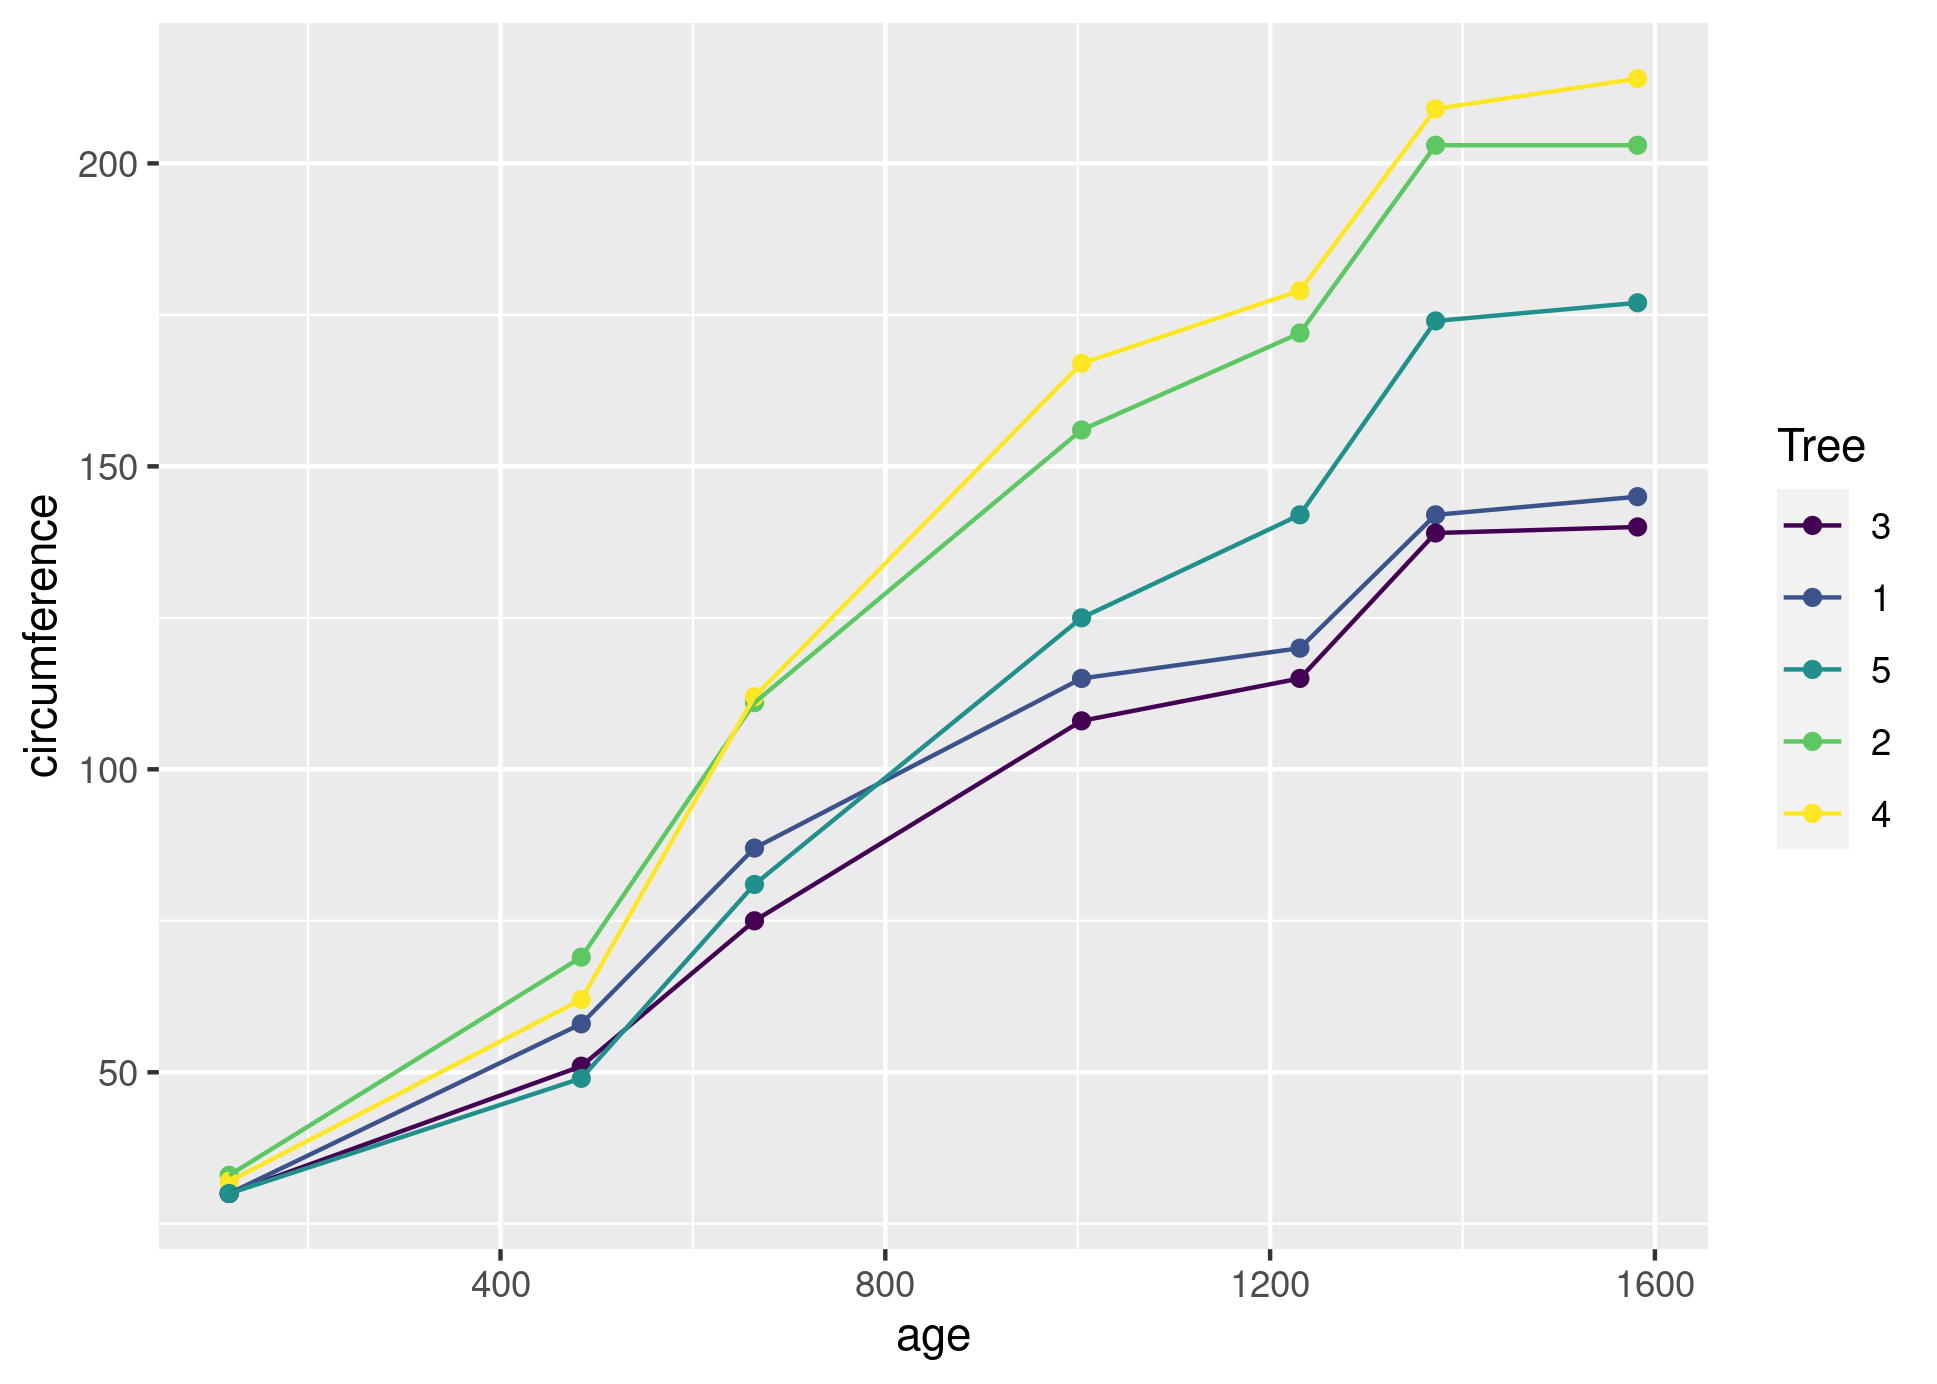
\includegraphics[width = 0.7 \linewidth]{figures/OrangeData.png}
 \end{frame}

 
%====================================================================
 \begin{frame}{Example 2: nlme}
%====================================================================
 
  \begin{columns}[t]
 \begin{column}{0.50\linewidth} 
  \begin{block}{}
   \begin{itemize}
  \item Logistic relation between $y$ and $t$
  $$ f(t;\phi) = \frac{a}{1+e^{-\frac{t-b}{c}}}$$
  \item  Gaussian noise
  \item Individual effect of each tree
 \end{itemize}
   
  \end{block}
\end{column}

  \begin{column}{0.50\linewidth} 
  \begin{block}{Latent variable model}
 
\begin{eqnarray*}
Y_{ij} &=& \frac{A + a_{i}}{1+e^{-\frac{t-(B+b_i)}{C+c_i}}} + \varepsilon_{ij}\\
\varepsilon_{ij} &\sim& \mathcal{N}(0,\sigma^2)\\
a_i &\sim_{i.i.d}& \mathcal{N}(0, \omega^2_a)\\
b_i &\sim_{i.i.d}& \mathcal{N}(0, \omega^2_b)\\
c_i &\sim_{i.i.d}& \mathcal{N}(0, \omega^2_c)
\end{eqnarray*}
   \end{block}
   \vspace{1em}
   
\end{column}
\end{columns}
 
 
 \begin{itemize}
  \item {\vert Latent variables} : $\ba  =  (a_1,\dots,a_5)$,$\bb = (b_1,\dots,b_5)$, $\bc = (c_1,\dots,c_5)$
  \item {\vert Parameters} :  $\theta = (A,B,C,\omega^2_a,\omega^2_b,\omega^2_c,\sigma^2)$
 \end{itemize}

 \end{frame}

%====================================================================
 \begin{frame}{Example 2: likelihood}
%====================================================================

{\small 
\begin{eqnarray*}
 p(\by | \ba,\bb,\bc;\theta) &=& \prod_{i=1}^5 \prod_{j=1}^{n_{i}} \frac{1}{2\pi \sqrt{\sigma^2}} \exp\left[-\frac{1}{2\sigma^2}\left(y_{ij}- f(t_{ij};A+a_i,B+b_i,C+c_i)\right)^2\right]\\
 p(\ba;\theta)  &=& \prod_{i=1}^5 \frac{1}{2\pi \sqrt{\omega_a^2}}  \exp\left[-\frac{1}{2\omega_a^2} a_i^2\right]\\
 p(\bb;\theta)  &=& \prod_{i=1}^5 \frac{1}{2\pi \sqrt{\omega_b^2}}  \exp\left[-\frac{1}{2\omega_b^2} b_i ^2\right]\\
 p(\bc;\theta)  &=& \prod_{i=1}^5 \frac{1}{2\pi \sqrt{\omega_c^2}}  \exp\left[-\frac{1}{2\omega_b^2} c_i^2\right]\\
  \ell(\by;\theta) &=& \int_{\ba,\bb,\bc} p(\by|\ba,\bb,\bc;\theta)p(\ba;\theta) p(\bb;\theta) p(\bc;\theta) d\ba\;  d\bb \;  d\bc 
\end{eqnarray*}}

\centering Not an explicit expression \color{dgreen} $\Rightarrow$ \color{black} Impossible to get an expression of the posterior distribution
 
 \end{frame}


%====================================================================
\begin{frame}{A few words on MCMC}
%====================================================================
 
\begin{itemize}
 \item Enabled the development of Bayesian inference in the  90's
 \item Stochastic algorithms
\end{itemize}

\begin{block}{Principle}
 \begin{itemize}
 \item  \vert Principle: \noir generates a Markov Chain  $\btheta^{(m)}$ whose ergodic distribution  (asymptotic, after a large number of iterations) is the distribution of interest  $[\btheta |\bY]$
 \item \vert What it will produce : \noir a sample  ($\btheta^{(1)} ,\dots, \btheta^{(M)}$) from the distribution $[\btheta | \bY]$
 \item \vert What will I do with it?  \noir  this sample supplies an approximation of the posterior distribution  (so : histograms, moments, quantiles...) 
 $$ \widehat{E[\btheta | \bY]} = \frac{1}{M}\sum_{m=1}^M \btheta^{(m)}$$
\end{itemize}

\end{block}


\end{frame}
 

 %====================================================================
 \subsection{Metropolis Hastings}
%====================================================================
\begin{frame}[allowframebreaks]{Metropolis-Hastings algorithm}
%====================================================================
\begin{itemize}
 \item  Belongs to the family of  {\vert M}onte {\vert C}arlo {\vert M}arkov {\vert C}hains
 \item \vert Idea\noir: explore the posterior distribution  with a random walk using a proposal distribution to move.
 \end{itemize}
 
 \begin{tabular}{ccc}
  
  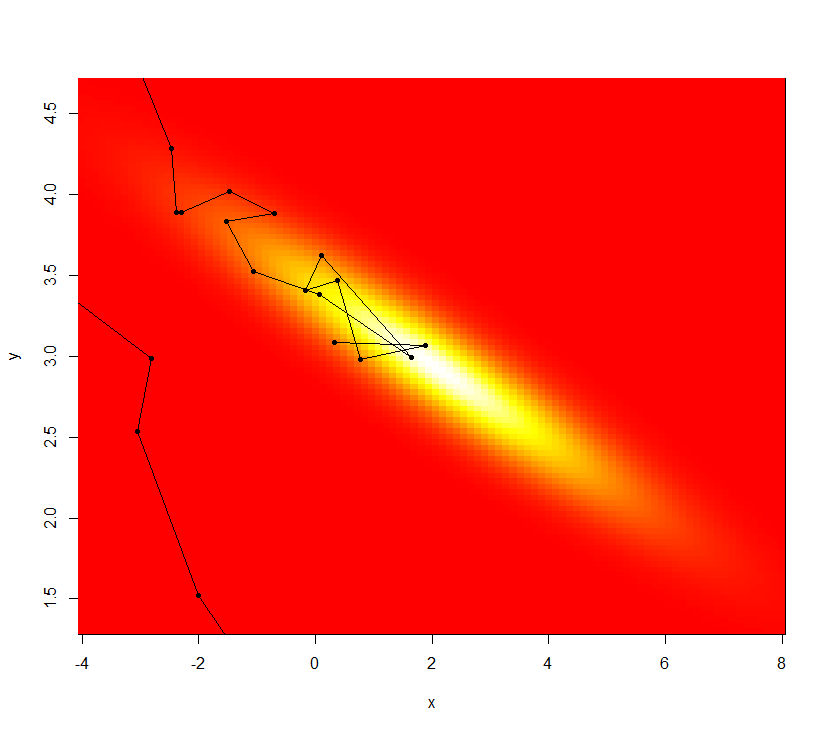
\includegraphics[width=0.3\textwidth]{figures/MCMC_chain_debut.png}&
  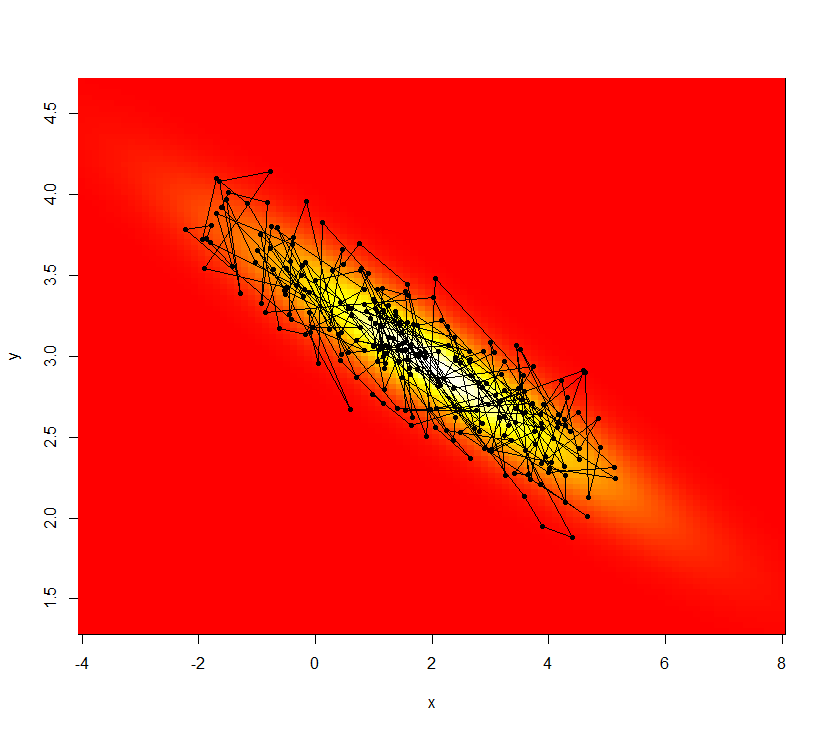
\includegraphics[width=0.3\textwidth]{figures/MCMC_chain_milieu.png}&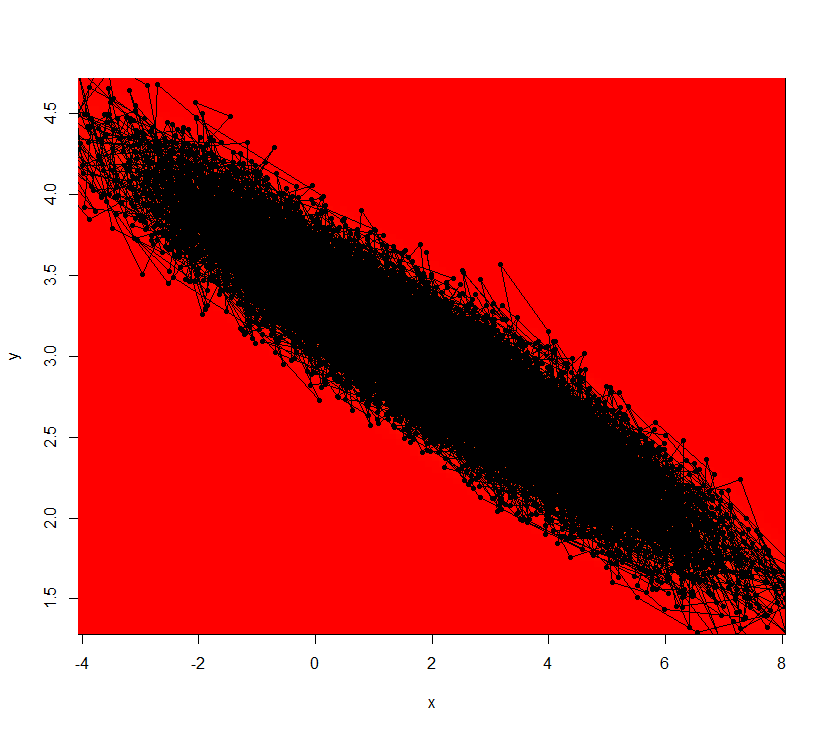
\includegraphics[width=0.3\textwidth]{figures/MCMC_plot_50000.png}
% 
 \end{tabular}

\begin{itemize}
 \item Let's chose an instrumental distribution  $q(\btheta' | \btheta)$  which can be easily simulated.  
  \end{itemize}
 
\begin{block}{A iteration $0$}
   Initialize  $\theta^{(0)}$ arbitrarily chosen  
\end{block}
     
     
 \begin{block}{At iteration  $m$}
 \begin{enumerate}
 \item Propose a candidate $\btheta^{c} \sim q(\btheta^{c} | \btheta^{(m-1)})$
 \item Calculate an acceptance probability :  
 $$ \rho(\btheta^c | \btheta^{(m-1)} )= \min\left\{1, \frac{[\btheta^{c} | \bY] }{[\btheta^{(m-1)}| \bY]} \frac{q(\btheta^{(m-1)} | \btheta^{c})}{q(\btheta^{c} | \btheta^{(m-1)})}\right\} $$
 \item  Accept the candidate with probability  $\rho(\btheta^c | \btheta^{(m-1)} )$, i.e. 
 $$u \sim \mathcal{U}_{[0,1]} \quad \mbox{et} \quad 
  \btheta^{(m)} = \left\{ \begin{array}{cl} \btheta^c & \mbox{ si } u<  \rho(\btheta^c | \btheta^{(m-1)} )\\
  \btheta^{(m-1)}  & \mbox{ sinon} 
  \end{array}
  \right.
  $$ 
\end{enumerate}
\end{block}
\end{frame}

  %====================================================================
 \begin{frame}{Why can I apply it?  }
 %====================================================================
  $$ \rho(\btheta^c | \btheta^{(m-1)} )= \min\left\{1, \frac{\vert [\btheta^{c} | \bY] }{\vert [\btheta^{(m-1)}| \bY]} \frac{q(\btheta^{(m-1)} | \btheta^{c})}{q(\btheta^{c} | \btheta^{(m-1)})}\right\} $$
  

\begin{eqnarray*}
 \frac{\vert [\btheta^{c} | \bY] }{\vert [\btheta^{(m-1)}| \bY]} &=& \frac{[\bY| \btheta^{c} ][\btheta^{c}]/\cancel{\vert [\bY]} }{[\bY| \btheta^{(m-1)} ][\btheta^{(m-1)}]/\cancel{\vert [\bY]}}\\
 &=& \frac{[\bY| \btheta^{c} ][\btheta^{c}]  }{[\bY| \btheta^{(m-1)} ][\btheta^{(m-1)}]}
 \end{eqnarray*}

 \begin{itemize}
  \item Easy to compute provided I know how to evaluate the likelihood
  \item Metropolis-Hastings :  universal (can be used in a large number of cases $=$ models)
   \end{itemize}
\vert 
\end{frame}

%====================================================================
 \begin{frame}{Random walk : particular choice of $q$}
 %====================================================================
  
 \vert Required qualities on $q$:  \noir  easy to propose a candidate: easy to  simulate, explicit probability density, with a support larger than the one of the distribution of interest 
 
 
 \begin{itemize}
 \item 
  $$ \theta^{c}  = \theta^{(m-1)} + \xi, \quad \quad \xi\sim \mathcal{N}_d(0_d, \tau^2 \mathbb{I}_d)$$
 %\item  where here  $\hat{\Sigma}$ is the asymptotic covariance matrix of the MLE  $\hat \btheta$
  \item In this case, symmetric kernel: $q(\btheta^{c} | \btheta^{(m-1)}) = q(\btheta^{(m-1)}| \btheta^{c} )$. 
  \end{itemize}
% \item \vert Example 2: independant kernel   \noir 
% $$q(\btheta^{c} | \btheta^{(m-1)})  =[\btheta^{c} ]$$  
 
 \begin{block}{Warning}
The choice of the transition kernel  $q(\cdot | \cdot)$ strongly influences the theoretical and practical convergence properties.  
\end{block}
\end{frame}
 
 
%====================================================================
\begin{frame}{Visualisation of the principle}
%====================================================================

We have a look at the wonderful interactive viewer by Chi Feng. 
\href{https://chi-feng.github.io/mcmc-demo/app.html?algorithm=RandomWalkMH&target=banana}{\beamergotobutton{chi-feng interactive MCMC}}


\end{frame}


%====================================================================
\begin{frame}{MH : convergence} 
%====================================================================
 \begin{itemize}
  \item By construction : $[\theta | \bY]$ is stationary 
  \item Explicit transition kernel
   $K(\theta' | \theta)$
  \item Prove that for any Borel set $A$
  $$ \int_{\theta' \in A} \int_\theta K(\theta'|\theta) p(\theta  | \by)  d\theta  d \theta' = \int_{\theta' \in A}p(\theta' | \by) d \theta'$$
 \end{itemize}
\end{frame}
%====================================================================
\begin{frame}{MH : kernel transition $K(\theta' | \theta)$} 
%====================================================================
Kernel transition such that
\begin{eqnarray*}
  \btheta^c &\sim& q(\btheta^c | \btheta)\\
  Z &\sim& \mathcal{B}ern(\alpha(\theta^c | \theta))\\
 \btheta' &=& Z \btheta^c    + (1-Z)  \btheta
 \end{eqnarray*}
 
Let's prove that  
  \begin{block}{}
$$K(\theta' | \theta) =   \alpha(\theta' | \theta) q(\theta'|\theta)  + r(\theta) \delta_{\theta}(\theta')$$
where
$$r(\theta) = \int_{\theta^c} (1-\alpha(\theta^c | \theta)) q (\theta^c | \theta) d \theta^c$$
\end{block}

 
\end{frame}
%====================================================================
 \begin{frame}{Kernel transition. Proof} 
%====================================================================
 For any measurable function $\phi$ we need $\mathbb{E}[\phi(\theta') | \theta]  = \int \phi(\theta')K(\theta' | \theta) d\theta'$

{\small 
\begin{eqnarray*}
 \mathbb{E}[\phi(\theta') | \theta]  &=&    \mathbb{E}_{\theta^c,Z}[\phi(Z \btheta^c    + (1-Z)  \btheta)] \pause \\ 
 &=&    \mathbb{E}_{\theta^c,Z}[Z \phi(\btheta^c)    + (1-Z)  \phi(\btheta)] \pause\\
&=& \int_{\theta^c} \left[\phi(\btheta^c)\mathbb{P}(Z = 1 | \theta) +  \phi(\btheta) \mathbb{P}(Z = 0 | \theta)\right] q(\btheta^c | \btheta) d \theta^c \pause \\ 
 &=&  \int_{\theta^c}  \phi(\btheta^c)\alpha(\theta^c | \theta) q(\btheta^c | \btheta) d \theta^c  + \phi(\theta)\underbrace{ \int_{\theta^c} (1-\alpha(\theta^c | \theta)) q (\theta^c | \theta) d \theta^c}_{r(\theta)} \pause\\
 &=& \int_{\theta'} \phi(\theta') \alpha(\theta' | \theta) q(\theta'|\theta)d\theta'  + r(\theta) \phi(\theta) \pause \\
&=&  \int_{\theta'} \phi(\theta')    \alpha(\theta' | \theta) q(\theta'|\theta)  + r(\theta) \int_{\theta'} \phi(\theta') \delta_{\theta}(\theta')  d\theta' \pause \\
&=&  \int_{\theta'} \phi(\theta')  \left\{ \alpha(\theta' | \theta) q(\theta'|\theta)  + r(\theta) \delta_{\theta}(\theta')\right\} d\theta'   
\end{eqnarray*}
 }



\end{frame}

%==================================================================== 
\begin{frame}{MH : stationarity}
%====================================================================


We have to prove that  for any subset $A$, 

$$ \int_{\theta' \in A}\int_{\theta} K(\theta' | \theta) p(\theta|y) d\theta d\theta'= \int_{\theta' \in A} p(\theta' | y) d\theta'$$
 
 
 
\end{frame}
 
 

%==================================================================== 
\begin{frame}{Proof of stationarity I}
%====================================================================


\begin{eqnarray*}
&& \int_{\theta' \in A}\int_{\theta} K(\theta' | \theta) p(\theta|y) d\theta d\theta'\\
&=& \iint_{(\theta,\theta') }\ind_{A}(\theta') \left[  \alpha(\theta' | \theta) q(\theta'|\theta)  + r(\theta) \delta_{\theta}(\theta')\right] p(\theta| y) d\theta d\theta'\pause\\
&=& \underbrace{\iint_{(\theta,\theta') }\ind_{A}(\theta')   \alpha(\theta' | \theta) q(\theta'|\theta) p(\theta| y) d\theta d\theta'}_{=B} \\
&& + \underbrace{\iint_{(\theta,\theta')}\ind_{A}(\theta') r(\theta) \delta_{\theta}(\theta') p(\theta| y) d\theta d\theta'}_{=C}\pause\\
\end{eqnarray*}
\end{frame}

%====================================================================
\begin{frame}[allowframebreaks]{Proof of stationarity II}
%====================================================================
We set 
$D  = \left\{(\theta,\theta') | p(\theta'|y) q(\theta|\theta') \leq p(\theta|y) q(\theta'|\theta)\right\}$
such that
$$
 \alpha(\theta' | \theta)  = \left\{
 \begin{array}{ll}
  \frac{ p(\theta'|y) q(\theta|\theta')}{p(\theta|y) q(\theta'|\theta)} & \forall(\theta,\theta') \in D\\
    1 &\forall(\theta,\theta') \in D^c
 \end{array}
 \right.
$$

 Note that $(\theta,\theta')\in D \Leftrightarrow (\theta',\theta)\in D^c$. 

We divide the $B=  \iint_{(\theta,\theta')}\ind_{A}(\theta')   \alpha(\theta' | \theta) q(\theta'|\theta) p(\theta| y) d\theta d\theta'$ term into two parts: 
\begin{eqnarray*}
 B &=& \iint_{(\theta',\theta) \in D }\ind_{A}(\theta')   \alpha(\theta' | \theta) q(\theta'|\theta) p(\theta| y) d\theta d\theta' \\
 && +\iint_{(\theta',\theta) \in D^c }\ind_{A}(\theta')   \alpha(\theta' | \theta) q(\theta'|\theta) p(\theta| y) d\theta d\theta'\pause \\
 &=&\underbrace{\iint_{(\theta',\theta) \in D }\ind_{A}(\theta')    \frac{ p(\theta'|y) q(\theta|\theta')}{\cancel{p(\theta|y)} \cancel{q(\theta'|\theta)}} \cancel{q(\theta'|\theta) }\cancel{p(\theta| y)} d\theta d\theta'}_{B_1}
 \\
 && +  \underbrace{\iint_{(\theta,\theta') \in D^c  }\ind_{A}(\theta' ) q(\theta' |\theta) p(\theta | y) d\theta d\theta' }_{B_2}
 \end{eqnarray*}
\end{frame}
%====================================================================
\begin{frame}{Proof of stationarity III}
%====================================================================
Using the fact that $(\theta,\theta')\in D \Leftrightarrow (\theta,\theta')\in D^c$. 
we make a variable change in $B_2$ : $(\theta,\theta') \rightarrow (\theta',\theta)$
\begin{eqnarray*}
 B &=& \underbrace{\iint_{(\theta',\theta) \in D }\ind_{A}(\theta')  p(\theta'| y)q(\theta|\theta') d\theta d\theta'}_{B_1} \\
 && + \underbrace{\iint_{(\theta',\theta) \in D }\ind_{A}(\theta)  p(\theta'| y) q(\theta |\theta') d\theta d\theta'}_{B_2}
\end{eqnarray*}



\end{frame}

%====================================================================
\begin{frame}{Proof of stationarity IV : about $C$}
%====================================================================


\begin{eqnarray*}
 C&=& \iint_{(\theta,\theta')}\ind_{A}(\theta') r(\theta) \delta_{\theta}(\theta') p(\theta| y) d\theta d\theta'\\
 &=& \int_{\theta}  r(\theta) \ind_{A}(\theta)p(\theta| y)  d\theta \\
 &=& \int_{\theta}  \left[ \int_{\theta'} \underbrace{\left(1-\alpha(\theta' | \theta)\right)}_{= 0,  \forall (\theta,\theta') \in D^c} q(\theta'|\theta) d\theta' \right] \; \ind_{A}(\theta)p(\theta| y)  d\theta\\ 
 &=& \iint_{(\theta,\theta') \in D} \left(1-\alpha(\theta' | \theta)\right)  q(\theta'|\theta)  \ind_{A}(\theta)p(\theta| y)  d\theta d\theta'\\
 &=& \underbrace{\iint_{(\theta,\theta') \in D}  q(\theta'|\theta)\ind_{A}(\theta)p(\theta| y)  d\theta d\theta' }_{C_1} \\
 && - \iint_{(\theta,\theta') \in D} \alpha(\theta' | \theta)   q(\theta'|\theta)\ind_{A}(\theta)p(\theta| y)  d\theta d\theta'  \quad  \quad (=B_2) 
\end{eqnarray*}

\end{frame}
%====================================================================
\begin{frame}{Proof of stationarity IV : conclusion}
%====================================================================
$$C = C_1 - B_2$$ 
\begin{eqnarray*}
C_1 &=& \iint_{ D}  q(\theta'|\theta)\ind_{A}(\theta)p(\theta| y)  d\theta d\theta' =   \iint_{D^c}  q(\theta|\theta')\ind_{A}(\theta')p(\theta'| y)  d\theta d\theta' 
\end{eqnarray*}
So 
{\small \begin{eqnarray*}
&& \int_{\theta' \in A}\int_{\theta} K(\theta' | \theta) p(\theta|y) d\theta d\theta' = B + C  = B_1 + \cancel{B_2} + C_1 - \cancel{B_2} \\
 &=& \iint_{  D }\ind_{A}(\theta')  p(\theta'| y)q(\theta|\theta') d\theta d\theta' +  \iint_{  D^c}  q(\theta|\theta')\ind_{A}(\theta')p(\theta'| y)  d\theta d\theta' \\
 &=& \iint \ind_{A}(\theta')  p(\theta'| y)q(\theta|\theta') d\theta d\theta'\\
 &=& \int_{\theta'} \ind_{A}(\theta') \underbrace{\int_{\theta} q(\theta|\theta')d\theta}_{=1}  p(\theta'| y)d\theta' = \int_A p(\theta'| y)d\theta'
 \end{eqnarray*}}
 \begin{flushright} 
cqfd
\end{flushright}
\end{frame}


%==================================================================== 
 \begin{frame}{Convergence}
 %====================================================================
 \begin{block}{Theoretical convergence }
 \begin{itemize}
  \item By construction : $[\theta | \bY]$ is stationary
  \item The theoretical convergence depends on the distribution of interest and the instrumental distribution  . \color{dgreen}  \cite{robert1999monte} \color{black}
 %\item For the random walk, Pour la marche aléatoire précédemment décrite, l'ergodicité est garantie si la loi d'intérêt est positive et  bornée sur tout compact de son support.  
\end{itemize}
\end{block}
\begin{block}{Practical convergence}
  
\end{block}
\end{frame}


 




  

%====================================================================
\begin{frame}[fragile]\frametitle{About the acceptance rate}
%====================================================================
 
 
 For the random walk
 $$ \theta^{c}  = \theta^{(m-1)} + \xi, \quad \quad \xi\sim \mathcal{N}_d(0_d, \tau^2 \mathbb{I}_d)$$
 

\begin{itemize}
\item $\tau$ small : we are moving very slowly in the parameters space because the steps are small. I accept a lot but I won't visit all the parameter space
\item $\tau$  big : we are moving slowly in the parameter space because the steps are big. The algorithm does not accept a lot, we are not moving enough 
\item $\tau$ medium' : we reach quickly the stationary distribution 
% \item \vert Practical strategy:  \noir
% \begin{itemize}
% \item Covariance structure $\Sigma$ coming from the MLE or from a first MCMC. 
% \item Heuristic based on theoretical works on gaussian distributions \cite{brooks}
% \item Tune $\tau$ to reach this acceptance rate
% 
% \end{itemize}
\end{itemize}
\end{frame}




%====================================================================
\begin{frame}[fragile]\frametitle{Trajectories  $(\btheta^{(m)})_{m\geq 0}$}
\centering
%====================================================================

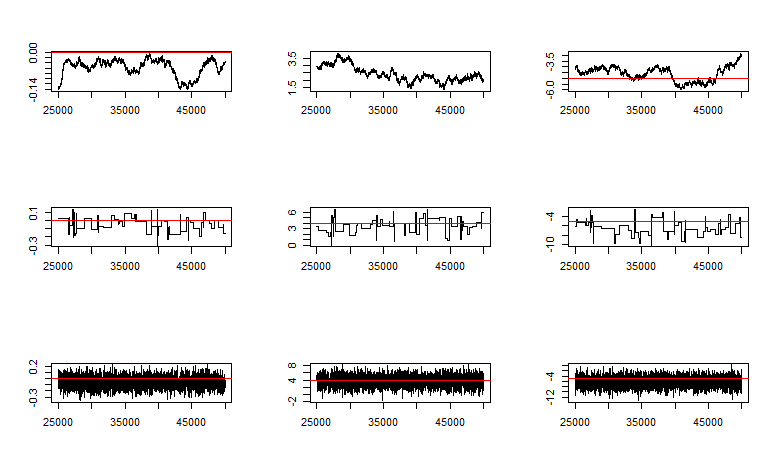
\includegraphics[width=\linewidth]{figures/probit_mcmc.png} 


Chains obtained for  $3$ values of  $\tau$ (resp. 0.01,1.5,10). We remove a burn-in period (25000 iterations over the total 50000 iterations)
\end{frame}


%====================================================================
\begin{frame}[fragile]\frametitle{Remarks}
 \begin{itemize}
  \item Target an acceptance rate of  25 \% in problems of small dimension, 50\% in large dimension problems. 
  \item Can also consider mixtures of kernels
$\rho_1 < \rho_2 < \rho_3$

$$\xi  \sim p_1 \mathcal{N}(0,\rho_1) + p_2 \mathcal{N}(0,\rho_2)+ (1-p_1-p_2) \mathcal{N}(0,\rho_3)$$
\item Be careful if the parameter leaves in a constrained set. 
\end{itemize}
\end{frame}


%====================================================================
\begin{frame}[fragile]\frametitle{Exercice}
 
Let us consider the Poisson regression : 
\begin{eqnarray*}
y_i &\sim& \mathcal{P}(\mu_i) \\
\log \mu_i &= & x_i \beta\\
\beta &\sim& \mathcal{N}(0, \sigma^2I_p) 
\end{eqnarray*}
 
\begin{itemize}
 \item Write (in R) a MCMC such that its asymptotic distribution is $p(\theta | y)$.
 \item Tune the size of the random walk to observe changes in the behavior
 \item See codes in \verb|BayesRegressionPoisson_MH.R|
\end{itemize}
  


 
\end{frame}



 




%====================================================================
\subsection[Gibbs]{Gibbs sampler} 
%==================================================================== 
\begin{frame}\frametitle{General Gibbs algorithm}
%====================================================================

If we want to sample a distribution  $p(\theta_1,\dots,\theta_d|\by)$  such that all the conditional distributions $g_j(\theta_1 | \theta_{\{-j\}},\by)$ are explicit, then the Gibbs algorithm is: 
\begin{block}{}
\begin{enumerate}
\item[] \vert Iteration 0:  \noir Initialize $\theta_1^{(0)} \dots, \theta_d^{(0)} $ 
\item[] \vert Iteration $m$ $(m=1\dots M)$: \noir  Given the current values of   $\theta_1^{(m-1)}, \dots, \theta_d^{(m-1)}$, 
\begin{itemize}
\item Simulate $\theta^{(m)}_1 \sim g_1(\theta_1 | \theta_2^{(m-1)}, \dots,x_d^{(m-1)},\by )$
\item Simulate  $\theta^{(m)}_2 \sim g_2(\theta_2 | \theta_1^{(m)}, \theta_3^{(m-1)}\dots,\theta_d^{(m-1)} ,\by)$
\item Simulate $\theta^{(m)}_3 \sim g_3(\theta_3 | \theta_1^{(m)},  \theta_2^{(m)}, \theta_4^{(m-1)}\dots,\theta_d^{(m-1)},\by)$
\item $\cdots$
\item  Simulate $\theta^{(m)}_d \sim g_d(\theta_d | \theta_1^{(m)}, \dots,\theta_{d-1}^{(m )},\by )$
\end{itemize}
\end{enumerate}
\end{block}
The stationary distribution is the joint one $p(\theta_1,\dots,\theta_p|\by)$



\end{frame}



%====================================================================
\begin{frame}\frametitle{Gibbs for latent variables}  
%====================================================================
Assume that we introduce latent variables $\bZ$ in the model such that   $[\bZ | \bY, \btheta]$ and  $[\btheta | \bY, \bZ]$  have an explicit form and can be easily simulated. 

\begin{block}{}
\begin{enumerate}
\item[] \vert Iteration 0:  \noir Initialise $\btheta^{(0)}$  et $\bZ^{(0)}$
\item[] \vert Iteration $m$ $(m=1\dots M)$: \noir  Given the current values of $\bZ^{(m-1)}$, $\btheta^{(m-1)}$
\begin{itemize}
\item Simulate $\bZ^{(m)} \sim [\bZ| \btheta^{(m-1)}, \bY]$
\item Simulate  $\btheta^{(m)} \sim [\btheta | \bZ^{(m)}, \bY]$
\end{itemize}
\end{enumerate}
\end{block}
We will get a sample of $(\bZ^{(m)}, \btheta^{(m)})_{m \geq 1}$ under the posterior distribution  $[\btheta, \bZ  | \bY]$ and so marginally $\btheta^{(m)} \sim [\btheta | \bY]$

\end{frame}

%====================================================================
\begin{frame}\frametitle{Exercice : Stationarity of $p(\theta,Z | Y)$}  
%====================================================================
\begin{enumerate}
 \item Explicit the kernel transition of the chain. 
 \item Prove that $p(\theta,Z | Y)$ is stationary.  
\end{enumerate}
\end{frame}

%====================================================================
\begin{frame}\frametitle{Convergence}  
%====================================================================
Ergodicity  and convergence studied in \cite{robert1999monte}.    

\end{frame}


%====================================================================
\begin{frame}\frametitle{Illustration : Gibbs sampler for a Poisson mixture model}
%====================================================================


\begin{itemize}
 \item  Mixture distribution 
 \begin{eqnarray*}
 Y_i &\sim&_{i.i.d.} \sum_{k=1}^K \pi_k \mathcal{P}(\mu_k)\\
  \end{eqnarray*}

\item Prior distribution
 \begin{eqnarray*}
 \mu_k &\sim& \Gamma(\alpha,\beta)\\
 \pi &\sim& \mathcal{D}ir(\nu, \dots, \nu)
 \end{eqnarray*}
 
\item Posterior distribution
$$[\pi, \mu_1, \dots \mu_K | Y] \propto \prod_{i=1}^n\left(\sum_{k=1}^K \pi_k e^{-\mu_k} \frac{\mu_k^{Y_i}}{Y_i!}\right) \prod_{k=1}^K\pi_k^{\nu-1}  \prod_{k=1}^K \mu_k^{\alpha-1} e^{-\beta \mu_k}
$$ 

\centering 

 \vert Not explicit
 
\end{itemize}
\end{frame}

%====================================================================
\begin{frame}\frametitle{Gibbs sampler for a Poisson mixture : latent variable version}
%====================================================================
\begin{itemize}
   \item Latent variables version
  \begin{eqnarray*}
 Y_i | Z_i = k &\sim&_{i.i.d.} \mathcal{P}(\mu_k)\\
 P(Z_i = k) &=& \pi_k\\
 (Z_{i1}, \dots,Z_{iK}) &\sim & \mathcal{M}(1, \pi) 
 \end{eqnarray*}
 with $Z_{ik} = \ind_{Z_i = k}$
 \item Conditional posterior distributions
\begin{equation*}
 \begin{array}{ccccl}
p(\mu,\pi | Y, Z) &\propto& p(Y,Z,\mu,\pi) &=& p(Y | Z, \mu) p(Z | \pi) p(\mu)  p(\pi)\\
p(Z | Y, \mu,\pi ) &\propto& p(Y,Z,\mu, \pi) &=& p(Y | Z, \mu) p(Z | \pi) \cancel{p(\theta)} \\
 \end{array}
\end{equation*}
\end{itemize}
\end{frame}

%====================================================================
\begin{frame}\frametitle{Gibbs sampler for a Poisson mixture: $p(\mu | Y,Z)$}
%====================================================================
 
 $$p(\mu | Y,Z) \propto p(Y | Z;\mu)   p(\mu)$$
 
 \begin{itemize} 
  \item \vert $ p(Y | Z, \mu)$ \noir 
 \begin{eqnarray*}
p(Y|Z,\mu) &=& \prod_{i=1}^n \frac{1}{Y_i!}e^{- \mu_{Z_i}} \mu_{Z_i}^{Y_i}\quad \pause  \propto \quad \prod_{k=1}^K \prod_{i=1,  Z_ik = 1}^n e^{- \mu_{k}} \mu_{k}^{Y_i}\pause \\
%&\propto&\prod_{k=1}^K  \left(e^{- \mu_{k}\sum_{i=1}Z_{ik}}\right)  \mu_{k}^{\sum_{i=1}Z_{ik}Y_i}\pause \\
&\propto&\prod_{k=1}^K e^{- \mu_{k}N_k}\mu_{k}^{S_k}
 \end{eqnarray*}
 with $N_k =\sum_{i=1}^nZ_{ik}$, $S_k = \sum_{i=1}^nZ_{ik}Y_i$ 
 
 \item \vert $p(\mu)$ \noir
 $$p(\mu) \propto \prod_{k=1}^K \mu_k^{\alpha-1} e^{-\beta \mu_k}$$
 
 \end{itemize}
 \end{frame}
 
%====================================================================
\begin{frame}\frametitle{Gibbs sampler for a Poisson mixture: $p(\mu | Y,Z)$}
%====================================================================
 
 $$p(\mu | Y,Z) \propto p(Y | Z;\mu)   p(\mu)$$
 
 
\begin{eqnarray*}
p(\mu | Y,Z) &\propto& \prod_{k=1}^K e^{- \mu_{k}N_k}\mu_{k}^{S_k}\prod_{k=1}^K \mu_k^{\alpha-1} e^{-\beta \mu_k}\\
&\propto& \prod_{k=1}^K e^{- \mu_{k}(N_k+\beta)}\mu_{k}^{\alpha + S_k-1}\\
\mu_k | Z,Y &\sim&_{i.i.d.} \Gamma(\alpha + S_k-1, N_k+\beta)
\end{eqnarray*}
 
\end{frame}
 
%====================================================================
\begin{frame}\frametitle{Gibbs sampler for a Poisson mixture: $p(\pi | Y,Z)$}
%====================================================================


$$ p(\pi | Y,Z) \propto  p(Z | \pi) p(\pi)$$

\begin{itemize}
\item \vert $ p(Z | \pi)$\noir 
   \begin{eqnarray*}
p(Z | \pi) &=& \prod_{i=1}^n \pi_{Z_i} \prod_{k=1}^K\prod_{i=1  | Z_{ik}=1}^n \pi_k \propto    \prod_{k=1}^K \pi_k^{N_k}
 \end{eqnarray*}
\item \vert $ p(\pi)$\noir 
$$p(\pi)\propto  \prod_{k=1}^K \pi_k^{\nu-1}$$
\item \vert $ p(\pi | Y,Z)  $\noir 
\begin{eqnarray*}
 p(\pi| Y,Z) &\propto& \prod_{k=1}^K \pi_k^{N_k + \nu-1}\\ 
 \pi  | Y,Z &\sim& \mathcal{D}ir(\nu +N_1, \dots, \nu + N_K)
\end{eqnarray*}
\end{itemize}
 \end{frame}

%====================================================================
\begin{frame}\frametitle{Gibbs sampler for a Poisson mixture: $p(Z | Y, \theta)$}
%====================================================================

\begin{itemize}
 \item 
\begin{eqnarray*}
p(Z | Y,\theta) &\propto&  p(Y | Z, \mu) p(Z | \pi) \\
&\propto& \prod_{i=1}^n e^{- \mu_{Z_i}} \mu_{Z_i}^{Y_i}  \pi_{Z_i}
\end{eqnarray*}
\item $Z_i$ independent conditionnally to $Y$ and $Z_i \in \{1, \dots, K\}$
\item 
\begin{eqnarray*}
   P(Z_i = k | Y,\theta)&\propto&  e^{- \mu_{k}} \mu_{k}^{Y_i}  \pi_{k}\\
   & = &  \frac{e^{- \mu_{k}} \mu_{k}^{Y_i}  \pi_{k}}{\sum_{k'=1}^K e^{- \mu_{k'}} \mu_{k'}^{Y_i}  \pi_{k'}}
\end{eqnarray*}
\end{itemize}
\end{frame}

 
%====================================================================
\begin{frame}\frametitle{Gibbs sampler for a Poisson mixture}
%====================================================================
\begin{block}{}
\begin{enumerate}
\item[] \vert Iteration 0:  \noir Initialize $\theta^{(0)}$  et $Z^{(0)}$
\item[] \vert Iteration $m$ $(m=1\dots M)$: \noir  Given current values of $Z^{(m-1)}$, $\theta^{(m-1)}$
 \begin{itemize}
 \item Simulate $ Z^{(m)} \sim [ Z| \theta^{(m-1)},  Y]$
 $\forall i=1,\dots,n$, $\forall g=1,\dots, G$
 \begin{eqnarray*}
   P(Z_i = k | Y,\theta^{(m-1)})&\propto&  e^{- \mu^{(m-1)}_{k}} (\mu^{(m-1)}_{k})^{Y_i}  \pi^{(m-1)}_{k}\\
  \end{eqnarray*}
%  }
 \item Simulate  $\theta^{(m)} \sim [\theta |  Z^{(m)},  Y]$
 {\scriptsize 
  \begin{itemize}
  \item  $N^{(m)}_k = \sum_{i=1}^n \ind_{Z^{(m)}_i=k}$ et  $S^{(m)}_{k} = \sum_{i=1}^n \ind_{Z^{(m)}_i=k}Y_{i}$
  \item  $ \mu^{(m)}_{k} | Z^{(m)},Y  \sim \Gamma\left(\alpha + S^{(m)}_{k}, b + N^{(m)}_k\right)$
  \item $ \pi^{(m)} | Z, Y  \sim \mathcal{D}ir(N^{(m)}_1 + \nu ,\dots,N^{(m)}_K + \nu) $
 \end{itemize}}
\end{itemize}
 \end{enumerate}
 \end{block}
  \end{frame}
  
%==================================================================== 
  \begin{frame}\frametitle{Exercice}
%====================================================================
Write the Gibbs corresponding to the SBM model
 $$Y_{ij} | Z_i = k, Z_j = l \sim \mathcal{P}(\mu_{kl})\quad , \quad P(Z_i = k) = \pi_k$$
\begin{enumerate}
 \item Write  the complete likelihood
 \item Propose prior distributions
 \item Calculate $P(\mu_{kl} | Y,Z)$
 \item Calculate $P(\pi | Y,Z)$
\item Are the $Z_i$'s independant conditionnally to $Y$? How will you proceed?  
 \end{enumerate}

  \end{frame}


%====================================================================
\begin{frame}\frametitle{Remarks on the Gibbs sampler}
%====================================================================
\begin{itemize}
\item For multidimensional distributions
\item Does not work if the number of parameters is variable % (ici, nombre de groupe $G$ fixé)
\item Constraining on the conditional distributions  (have to be explicit)
\item No tuning of the algorithm: + and -
\end{itemize}


\vspace{1em}


\color{dgreen}{Visualization}
\href{https://chi-feng.github.io/mcmc-demo/app.html?algorithm=GibbsSampling&target=banana}{\beamergotobutton{chi-feng interactive MCMC (Gibbs)}}
\end{frame}

  


%====================================================================
\subsection{Metropolis-Hastings within Gibbs}   
%====================================================================


%====================================================================
\begin{frame}\frametitle{Metropolis-Hastings within Gibbs} 
%====================================================================

 Convenient for latent variable models. Gibbs and Metropolis-Hastings combined
 
 \begin{block}{}
\vert Iteration 0:  \noir Initialise $\theta^{(0)}$  et $\bZ^{(0)}$\\

\vert Iteration $m$ $(m=1\dots M)$: \noir  Given the current values of $\bZ^{(m-1)}$, $\theta^{(m-1)}$
\begin{itemize}
 \item On the latent variables $\bZ$
        \begin{itemize}
        \item Propose $\bZ^{(c)} \sim q(\bZ| \bZ^{(m-1)},\theta^{(m-1)})$
        \item Accept with probability such that $[\bZ  |\theta  , \bY]$ is the stationary distribution 
        \end{itemize}
\item For each component of $\theta$
         \begin{itemize}
          \item Propose $\theta_k^{(c)} \sim q(\theta_k| \theta^{(m-1)}_{-\{k\}}, \bZ^{(m)})$
            \item Accept with probability such that $[\theta_k |\theta_{-\{k\}}, \bZ, \bY]$ is the stationary distribution  %$\theta_k \sim [\theta | \bZ^{(m)}, \bY]$
        \end{itemize}
\end{itemize}
\end{block}
We will get a sample of $(\bZ^{(m)}, \theta^{(m)})_{m \geq 1}$ under the posterior distribution  $[\btheta, \bZ  | \bY]$ and so marginally $\theta^{(m)} \sim [\theta | \bY]$

 \end{frame}
  
%====================================================================
 \begin{frame}{ Great but and now...}
%==================================================================== 
 \begin{itemize}
  \item Many packages to automatically construct the MCMC from your model. 
  \item Very flexible and adapted to latent variable models
  \item Based on the writing of the model : automatically designed proposals
 \end{itemize}
 
  \end{frame}
  
%====================================================================
\begin{frame}{Software}
%====================================================================
\begin{itemize}
  \item \href{http://www.mrc-bsu.cam.ac.uk/software/}{WinBUGS} : Bayesian inference Using Gibbs Sampling for Windows.  `Point-and-click’ windows interface version. May also be called from   
\includegraphics[width=0.05\linewidth]{figures/Rlogo-1.png}.  
  \item  With    
\includegraphics[width=0.05\linewidth]{figures/Rlogo-1.png} : package \textsf{R2WinBUGS}
  \item  \href{http://www.openbugs.net/w/FrontPage}{OpenBUGS} 
 \item \href{http://mcmc-jags.sourceforge.net/}{JAGS} : Just An Other Gibbs Sampler. More recent.From   
\includegraphics[width=0.05\linewidth]{figures/Rlogo-1.png}: r2JAGS or rJAGS...
 \item \href{https://mc-stan.org/}{STAN} : developed by Andrew Gelman, coding more complex but more powerful. 
 \end{itemize}
  
 \end{frame}
 
%====================================================================
\begin{frame}{In pratice}
%====================================================================
 \centering

Have a look at the file  
exempleLinearModelIrispresentation.html

 

  
\end{frame}
  
%====================================================================
\subsection{Tuning and assessing the convergence of MCMC}
%====================================================================
\begin{frame}{Tunning}
 
\begin{itemize}
 \item As we saw : step-size will have a non-neglectable influence on the convergence. 
 \item Solution : run the algorithm for a few iterations, check the acceptance rate 
\begin{itemize}
  \item If the acceptance rate is too low, decrease the step-size. 
  \item If the acceptance rate is too high, increase the step-size. 
\end{itemize}
\item \color{dgreen} \textbf{Be careful}\color{black}: not possible to adapt the acceptance rate   along the iterations, because in that case, it would not be a Markov Chain anymore (theoretical convergence conditions do not hold anymore)
\end{itemize}
\end{frame}


%====================================================================
\begin{frame}{Burn-in}
%====================================================================
\begin{itemize}
 \item Period where the chain will reach the stationary distribution
 \item Need to remove the first iterations (check the traces to calibrate)
\end{itemize}
 
\end{frame}
%====================================================================
\begin{frame}{Thinning}
 %====================================================================
\begin{itemize}
 \item With our sample $\theta^{(1)}, \dots, \theta^{(M)}$ we want to compute expectations, kernel density estimates of the posterior, etc...
 $$ \frac{1}{M}\sum_{m=1}^M \phi(\theta^{(m)})$$
 \item The convergence of such estimates is ensured (LGN) if the $\theta^{(m)}$ are independent and identically distributed.  
 \item In our case : $\theta^{(m)}$ realisations of a Markov Chain, so not independent. 
 \item To break the dependence, \color{dgreen} \textbf{thin}\color{black}: take one realization over ... (to be set). 
 \end{itemize}

\end{frame}
%====================================================================
\begin{frame}{Number of iterations}
%====================================================================
Must take into account

\begin{itemize}
 \item The complexity of the model (number of parameters to sample)
 \item The burn-in period you need
 \item The thinning parameter you need
 \item The time you have
\end{itemize}
From 10000 to \dots  millions?
\end{frame}
%====================================================================
\begin{frame}{Assessing convergence}
%====================================================================
\begin{itemize}
 \item Plot of the chains, parameter by parameter
 \item Plot the autocorrelations plots
 \item Compute numerical indicators
\end{itemize}

\end{frame}
%====================================================================
\begin{frame}{Gelman-Rubin convergence diagnostic}
%====================================================================
\begin{itemize}
 \item Relies on several chains run in parallel
 \item Let $c$ be the index for the chain. 
  \item Must be initialized from \emph{over dispersed initial values $\theta^{c(0)}$} with respect to the targeted distribution. 
  \item Formulae compare the variances intra and inter chains
   \begin{itemize}
  \item Within-chain variance  averaged over the chains:
  $$s^2_c = \frac{1}{M-1}\sum_{m=1}^M (\theta^{c(m)}- \overline{\theta^{c}})^2 \quad W = \frac{1}{C}\sum_{c=1}^C s^2_c$$
  \item Between-chain variance:  $$B = \frac{M}{C-1} \sum_{c = 1}^C (\overline{\theta^{c}} - \overline{\overline{\theta}})^2$$  
  \item Variance of $\theta | y$ is estimated as a weighted mean of these two quantities
  $$\widehat{\mbox{var}}\!(\theta|y)
= \frac{M-1}{M}\, W \, + \, \frac{1}{M} \, B.$$ 
\item \emph{Potential scale reduction statistic} is defined by
$$\hat{R}
\, = \,
\sqrt{\frac{\widehat{\mbox{var}}\!(\theta|y)}{W}}.$$

\item If all chains are at equilibrium $\hat{R} \approx 1$. Otherwise, if the chains have not converged to a common distribution, the  
$\hat{R} \geq 1$
\item \fbox{Compare $\hat{R}$ with $1.1$.}
\end{itemize}
\end{itemize}
\end{frame}
%====================================================================
\begin{frame}{Geweke convergence diagnostic}
%====================================================================
\begin{itemize}
 \item  Perform a test on two parts of the chain. 
 \item Assume that the chain is of $M$ iterations
 \item Take $M\alpha_1$  first iterations and $M \alpha_2$ last iterations (such that $\alpha_1 + \alpha_2 <1$  
\item Compute the mean of $\theta$ on the two parts
 \item If we are at the stationary distribution, then the two means should be equal
 \item Correction by the variances (taking into account the dependance between the realisations
 \item Geweke is the $Z$-statistic of the test.
 \item A z-score higher than the absolute value of 1.96 is associated with a p-value of < .05 (two-tailed). The absolute value of $Z$ should therefore be lower than  1.96.
 \end{itemize}
\end{frame}
